\chapter{Software}
\label{chap:software}

The third chapter of this thesis describes the web application, CryptoShow, which is developed to provide a user-friendly interface for the methodology described in Chapter~\ref{chap:methodology}. This chapter covers the architecture, technologies used, backend and frontend development, testing, monitoring, and deployment of the application.

\section{Architecture and Used Technologies}
\label{sec:architecture-technologies}

This section outlines the architecture of the CryptoShow application and the technologies employed in its development. The application is designed to be modular and scalable, allowing for easy integration of new features and improvements. For this purpose, we have chosen a service-oritented architecture (SOA) that separates the components, enabling independent development and deployment. The architecture is defined by several Docker containers, each responsible for a specific part of the application. The services are orchestrated using Docker Compose, defined in the \texttt{docker-compose.yml} file, which specifies the services, networks, and volumes required for the application to run. The service architecture is as follows:

\begin{itemize}
    \item \textbf{backend} - Acts as the central API service, facilitating communication between most components. It communicates with Redis, manages API requests from the frontend, and delegates asynchronous tasks to Celery workers. The FastAPI server serves as its entry point. Further details are provided in Section~\ref{sec:backend}.
    \item \textbf{worker-cpu / worker-gpu} - These two services execute asynchronous, resource-intensive tasks without blocking the main FastAPI event loop. \texttt{worker-cpu} runs on the CPU, while \texttt{worker-gpu} leverages GPU acceleration via CUDA when available.
    \item \textbf{frontend} - Delivers the user interface. NginX acts as the gateway to the defined services in Docker Compose and serves static content from a specified directory. Additional information is available in Section~\ref{sec:frontend}.
    \item \textbf{redis} - Functions as the message broker for Celery workers, enabling efficient task distribution.
    \item \textbf{monitoring-flag} - A lightweight service that creates a flag file to enable the monitoring proxy endpoint.
    \item \textbf{remove-monitoring-flag} - A lightweight service that removes the monitoring flag file, disabling the monitoring endpoint.
    \item \textbf{flower} - Provides real-time monitoring and statistics for Celery tasks and queues.
    \item \textbf{celery-exporter} - Exposes Celery metrics to Prometheus, similarly to the Flower service.
    \item \textbf{prometheus} - Collects and stores metrics exported from the Celery workers.
    \item \textbf{grafana} - Offers a user-friendly dashboard for visualizing metrics collected by Prometheus.
\end{itemize}

\begin{figure}[htpb]
    \centering
    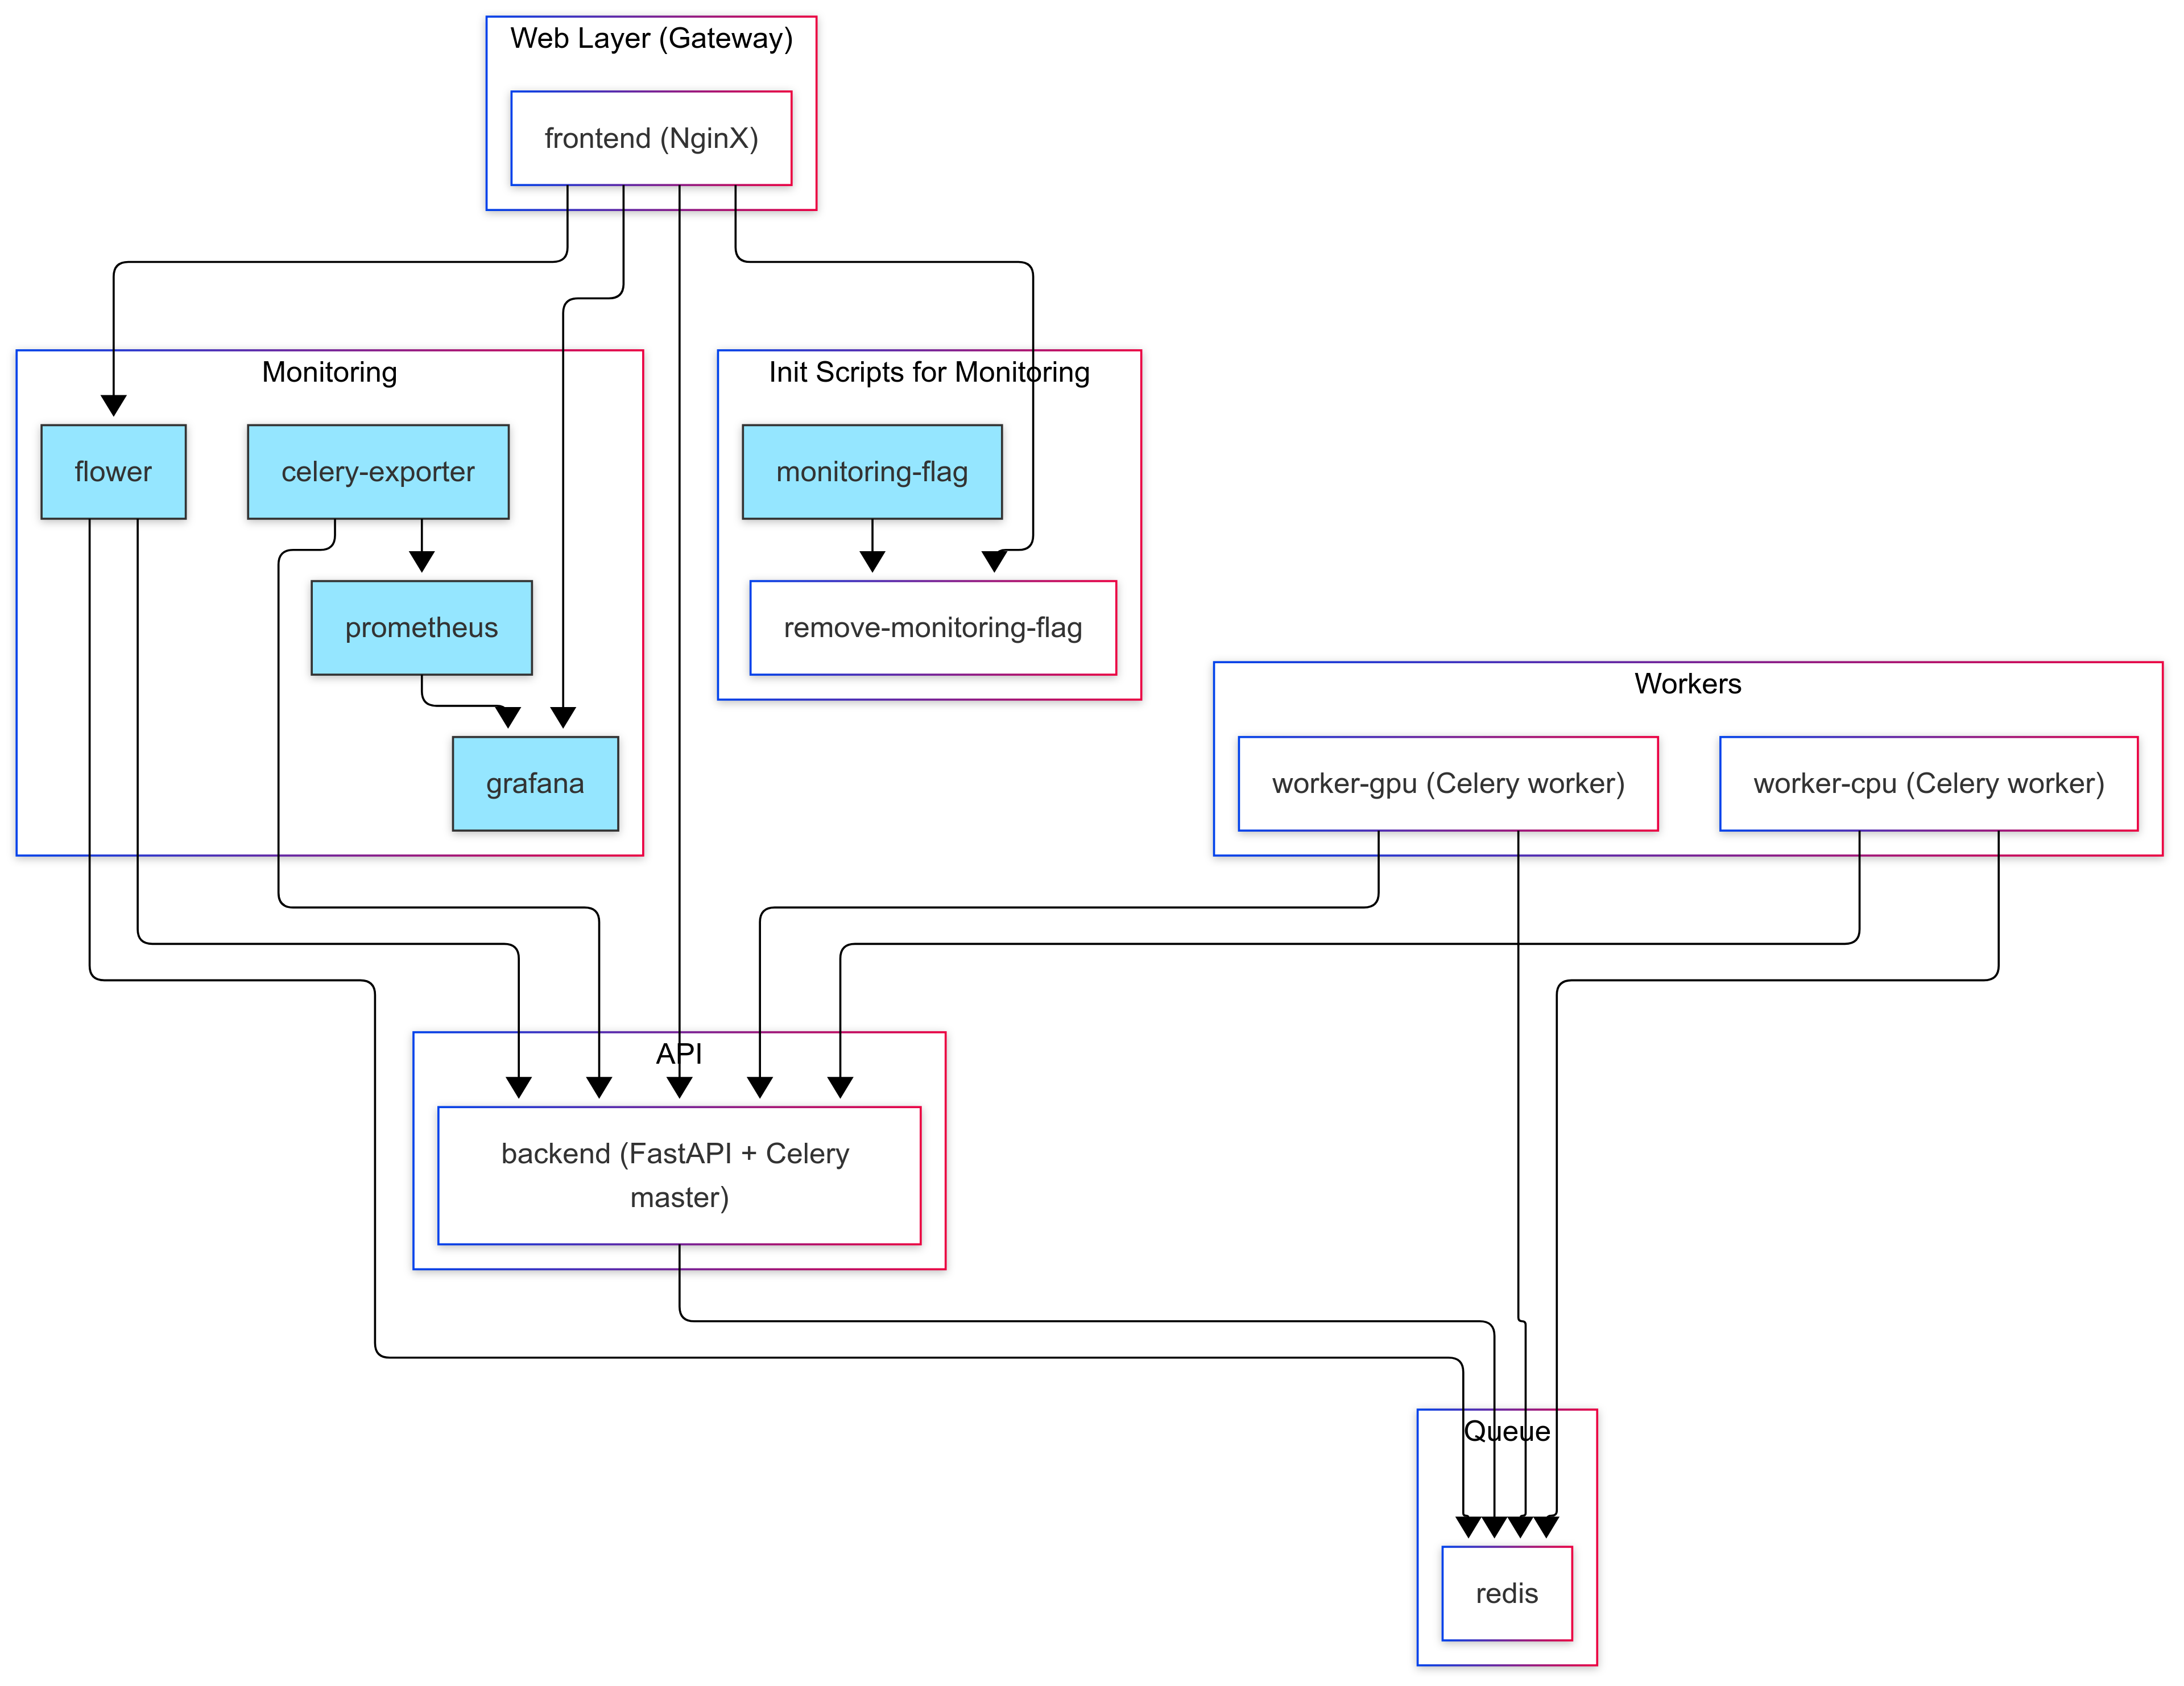
\includegraphics[width=\textwidth]{img/architecture.png}
    \caption{Service architecture of the CryptoShow application. Each small box represents a Docker containerized service. Light blue services are optional, as monitoring is not always required. Arrows indicate communication paths between services. Generated using the Mermaid Chart tool, available at \url{https://www.mermaidchart.com/}.}
    \label{fig:architecture}
\end{figure}

An overview of the service architecture can be seen in Figure~\ref{fig:architecture}. This type of architecture offers a scalable solution that has the potential of easy deployment and development.

Let's also focus on the technology stack for some of the services:

\begin{itemize}
    \item \textbf{backend, worker-cpu / worker-gpu} - Python, notable libraries and tools: Celery (asynchronous tasks in Python), FastAPI, Flower, PyTorch, BioPython, Biotite, Scikit-Learn, MDAnalysis, Gemmi, Redis, uv
    \item \textbf{frontend} - TypeScript, notable libraries, tools and frameworks: React, NginX, Mol*, Bun, Vite
\end{itemize}

The remaining services utilize standard technology stacks commonly associated with their respective functionalities.

\section{Backend}
\label{sec:backend}

The backend of the CryptoShow application is responsible for the core functionalities, such as calculating the predictions, clustering and smoothing the results, generating trajectory animations for AHoJ results, and serving the API endpoints for the frontend. This chapter provides an overview of the backend architecture.

This section covers the \textbf{backend, worker-cpu, worker-gpu} and \textbf{redis} services. All source codes can be found in the \lstinline!backend! directory.

All backend services utilize the same initial Dockerfile with one Python environment. This ensures consistency and speeds up the build process. For the installation of the Python environment, we use the \lstinline!pyproject.toml! file, which contains all necessary dependencies for the backend services, and is installed using the \lstinline|uv| tool\footnote{Available at \url{https://github.com/astral-sh/uv}.}. After installing the Python environment, the entrypoint for the backend service is run, which first checks for the presence of the machine learning models and downloads them if they are not available. Subsequently, the FastAPI server is started running on port 5000.

\subsection{FastAPI}
\label{sec:fastapi}

The backend service is built using FastAPI, a modern web framework for building APIs with Python\footnote{Available at \url{https://github.com/fastapi/fastapi}.}. It serves as the main entry point for the application, handling API requests and delegating tasks to Celery workers\footnote{Available at \url{https://github.com/celery/celery}.}.

FastAPI is chosen for its performance and ease of use, including the option to automatically generate OpenAPI documentation. The server includes configuration for CORS (Cross-Origin Resource Sharing), logging and error handling. The API contains several endpoints, including endpoints for health check, prediction for a given PDB ID, prediction for a custom protein structure, Celery task status check, and trajectory animation generation. To improve performance, WebSockets are used to check the status of the tasks, allowing the frontend to receive updates without polling the server.

\xxx{TODO: do we include all API endpoints? we can list them but I think it's not necessary to do so}

To support asynchronous task execution without blocking the main event loop, the backend service uses Celery workers. These workers are responsible for executing resource-intensive tasks, such as running the CB-Model, smoothing model and generating trajectory animations. The workers can run on either CPU or GPU, depending on the availability of resources (covered in detail in \ref{sec:deployment}). The backend service communicates with Redis, which acts as a message broker for Celery, allowing efficient task distribution and management.

The logic for the API endpoints is implemented in the \lstinline!backend/main.py! file.

\subsection{Prediction and Clustering}
\label{sec:prediction-backend}

To begin with the prediction, the necessary dependencies for the CryptoBench model must be installed. Once the Python environment is set up (this is done in Docker automatically), the Celery task is added to the queue. The task is defined in the \lstinline!backend/tasks.py! file, which is responsible for executing the prediction logic.

First, the structure provided by the user (either in the form of an ID or a custom structure) is processed and parsed using specialized parsers for the PDB/mmCIF formats (see Section~\ref{sec:pdb-format} and Section~\ref{sec:mmcif-format}). Only the first model of the structure is considered, as the CryptoBench model is designed to work with single-model structures. After parsing, the structure is then converted to a protein sequence, saved to FASTA files (see Section~\ref{sec:fasta-format}) for each chain, which is required for the prediction.

Afterwards, the fine-tuned ESM-2 model (\lstinline!facebook/esm2_t33_650M_UR50D!) is loaded, followed by the corresponding weight file from the Tiny-CryptoBench repository. The protein sequence is then tokenized using the ESM-2 tokenizer, segmented into chunks of 1022 tokens (1024 minus two special tokens), and processed by the CryptoBench model to obtain predictions. These predictions are subsequently concatenated to produce a single prediction vector representing the entire sequence. The model consists of three linear layers, two dropout layers, and a ReLU activation function. Then, the predictions are generated by applying the sigmoid activation function to the output of the final linear layer, resulting in a vector of probabilities for each residue in the sequence. The implementation for this procedure is provided in the \lstinline!backend/prediction/compute_score.py! file. The code is intended for use with individual protein sequences, as it requires parsing and splitting the sequence by chain to ensure accurate predictions.

After receiving the predictions for individual chains, 3D coordinates of all residues are extracted from the input structure. This step is required for the clustering and smoothing processes. The predictions are first clustered using the methodology described in Section~\ref{sec:clustering}. After clustering, the clusters are further smoothed. All source codes for the clustering and smoothing processes can be found in the \lstinline!backend/clustering! directory and follow the described methodology.

Following this refinement process, all collected data is collected into a single JSON object, which is subsequently stored, returned, and used by the frontend for result visualization.

\subsection{Trajectory Animation}
\label{sec:trajectory}

CryptoShow aims not only to predict and visualize cryptic binding sites, but also to demonstrate potential conformational changes through animated trajectories. To achieve this, we have developed a trajectory animation feature that illustrates structural transitions between related protein conformations.

Let us begin by introducing AHoJ \cite{feidakis2022ahoj} and AHoJ-DB \cite{feidakis2024ahoj} (briefly covered in Section \ref{sec:ahoj}). Apo–Holo Juxtaposition (AHoJ) is a web-based tool designed to identify apo-holo pairs of protein structures within the PDB database (Section~\ref{sec:rcsb-pdb}); currently, querying is limited to this database only.

AHoJ identifies binding residues by spatially marking user-defined ligands using PyMOL (Section~\ref{sec:pymol}). The tool compiles candidate structure chains by detecting UniProt accession numbers and retrieving all chains belonging to the same UniProt AC (Section~\ref{sec:uniprot-db}). It maps binding residues onto the UniProt sequence and examines each candidate chain to determine the presence of mapped binding residues above a minimum threshold. Successful candidates are aligned to the query chain using TM-align \cite{zhang2005tm}, and the area around the superimposed query ligand is examined for ligands. The process classifies each candidate chain as apo or holo based on ligand presence or absence in the defined binding sites, with results visualized in the browser and downloadable for PyMOL analysis. AHoJ-DB is a database of pre-computed apo-holo pairs of protein structures.

For CryptoShow's trajectory animation functionality, we make use of the AHoJ public API to identify apo-holo structural pairs corresponding to the input structure. The query process requires the PDB ID of the input structure\footnote{As mentioned above, AlphaFold structures and custom structures are not supported by AHoJ. Additionally, the input structure may be in holo form. This is not validated in any way. Apo structures are generally more appropriate for this analysis, we leave this decision on the user as it does not affect the functionality of CryptoShow.}, the target chain containing the predicted cryptic binding site, and the central residue of the identified CBS. Listing \ref{lst:ahoj-query} demonstrates the query format. The API response contains all available paired structures, from which users can select any structure to visualize potential conformational transitions. Upon selection, the CryptoShow API initiates the trajectory computation.

\begin{lstlisting}[caption={Sample query format for the AHoJ tool, specifying PDB ID 2src, chain A, aspartic acid residue at position 404}, label={lst:ahoj-query}]
    2src A ASP 404
\end{lstlisting}

First, the target structure for animation is downloaded from AHoJ. Both structure files are then converted to PDB format to ensure each contains only a single model and to allow easier manipulation compared to the mmCIF format (see Section~\ref{sec:pdb-format} and Section~\ref{sec:mmcif-format}). Subsequently, the PDB file is processed using the MDAnalysis library \cite{gowers2019mdanalysis}, from which the sequence and corresponding residues are extracted. At this point, we have obtained the necessary structural information.

Next, we need to determine which residues should be included in the animation. To achieve this, we employ a straightforward approach by computing the longest common subsequence of both protein sequences \xxx{TODO: should I add pseudocode here? it's not really that hard...}. This ensures that only residues present in both structures are animated. The subsequence length must be greater than zero due to the inherent logic of AHoJ. Once the common subsequence is identified, we extract the corresponding residues from both structures. We utilize the MDAnalysis library to perform this operation at the atomic level, as PDB files store coordinates for individual atoms rather than residues. Additionally, we extract all ligands from both structures to include them in the final animation.

In the end, we generate the trajectory using cubic spline interpolation \cite{mckinley1998cubic} implemented in the SciPy library \cite{virtanen2020scipy}. We create a trimmed PDB file containing only the relevant residues and ligands, along with a trajectory file featuring interpolated coordinates across a predetermined number of frames (set arbitrarily to 50). The final visualization presents the original structure at 50\% opacity and the target holo structure at full opacity, as illustrated in Figure \ref{fig:trajectory-animation}.

\begin{figure}[htbp]
    \centering
    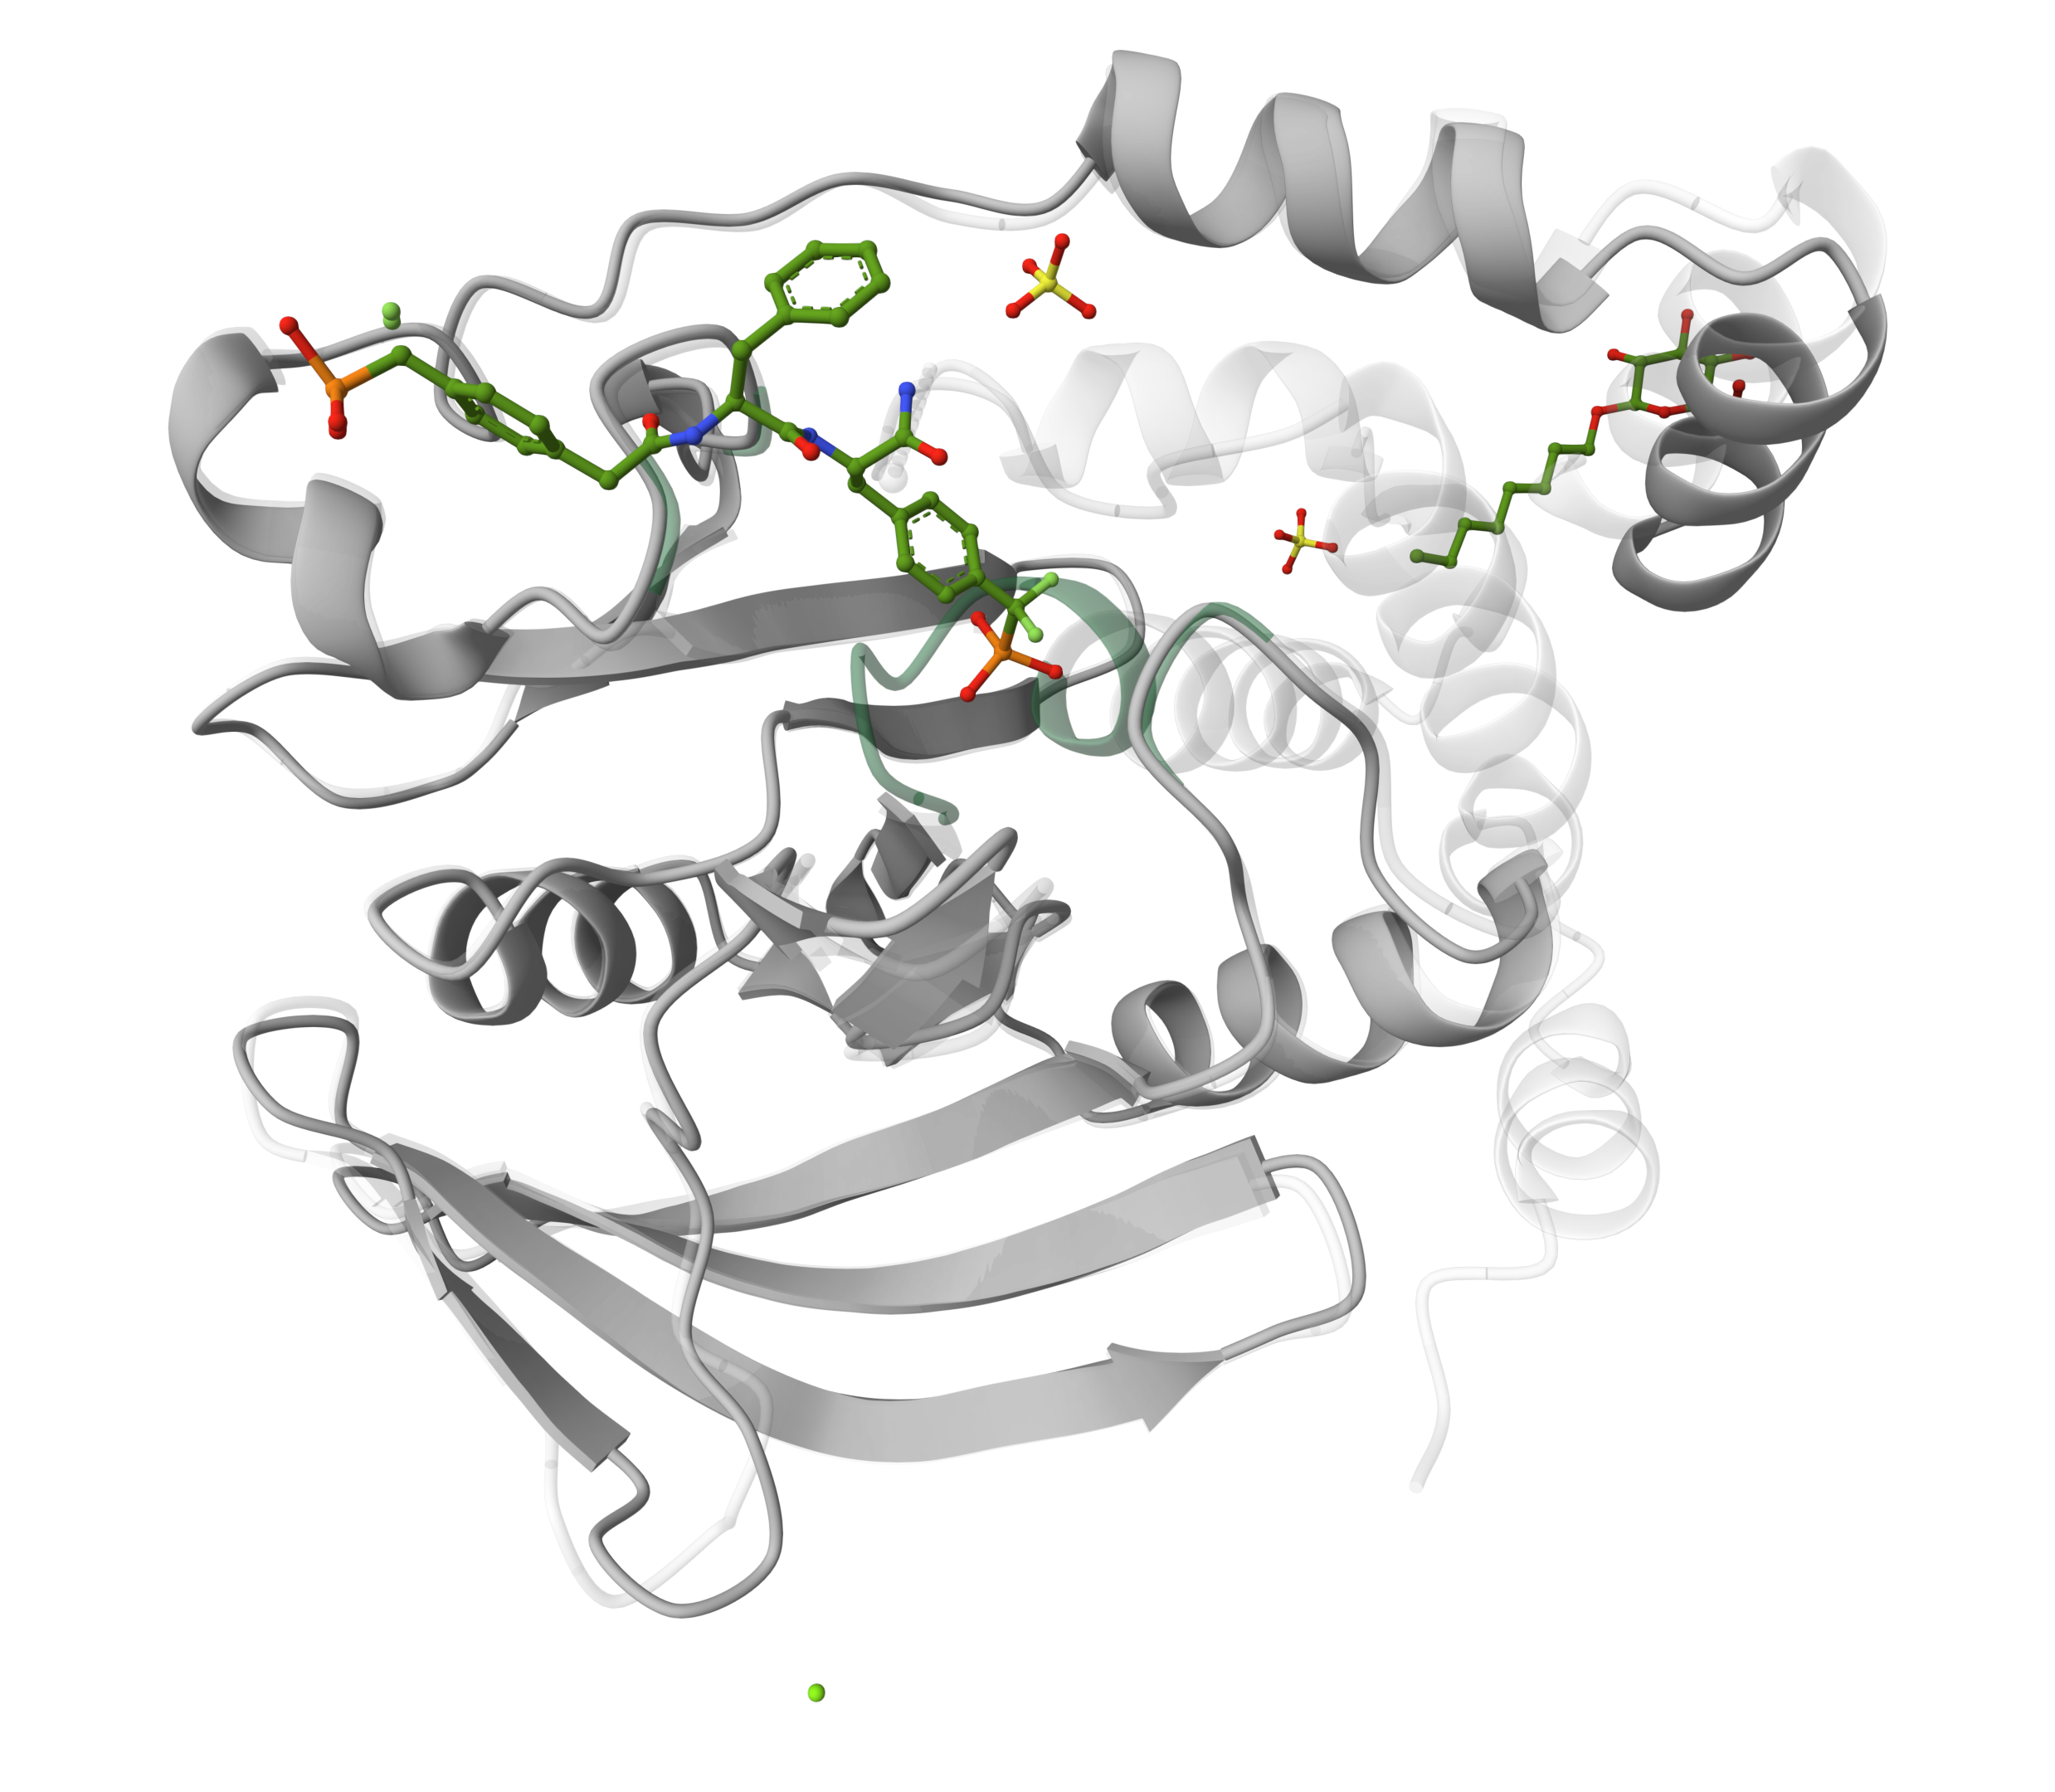
\includegraphics[width=\textwidth]{img/trajectory_animation.png}
    \caption{Example of trajectory animation demonstrating conformational changes between the input structure 1PTY (Crystal Structure of Protein Tyrosine Phosphatase 1B Complexed with Two Phosphotyrosine Molecules) and 2CNE (Structural Insights into the Design of Nonpeptidic Isothiazolidinone - Containing Inhibitors of Protein Tyrosine Phosphatase 1B). The input structure is displayed with 50\% transparency, while the target holo structure is rendered at full opacity. The ligand is represented in ball-and-stick format. Visualized using Mol* in CryptoShow.}
    \label{fig:trajectory-animation}
\end{figure}

Although this process generates a trajectory, it is important to note that this represents only a simple interpolation of residue coordinates. The trajectory does not depict actual conformational changes, but rather provides a smooth transition between the two structures. To capture genuine conformational dynamics, one would need to perform molecular dynamics simulations, which are computationally intensive and require significant time investment \cite{schlitter1993targeted}.

The source code for the trajectory animation functionality can be found in the \lstinline!backend/trajectory_generator! directory. As with the prediction and clustering components, the implementation details in the actual pipeline will be covered in Chapter \ref{chap:software}.


\section{Frontend}
\label{sec:frontend}

The frontend of the CryptoShow application is designed to provide an intuitive and user-friendly interface for the pipeline described in Chapter~\ref{chap:methodology}. The main technologies used for the frontend development include TypeScript, React, and Mol* (see Section~\ref{sec:molstar}), which is a powerful molecular visualization library. 

\subsection{NginX}
\label{sec:nginx}

The main component is NginX \cite{reese2008nginx}, which serves as a reverse proxy to many services and serves as one endpoint for the frontend. There are multiple configurations for NginX, which are defined in the \lstinline!frontend/nginx! files. We want to serve the frontend application in all cases, which is described by the default configuration. However, to improve user experience, we also provide configurations for TLS/SSL encryption, which is recommended for production environments. Moreover, we provide a configuration for the monitoring proxy endpoint, which is used to monitor the Celery tasks and queues (more details in Section~\ref{sec:tests-monitoring}). The NginX server listens on port 80 for HTTP requests and port 443 for HTTPS requests. The configuration files specify the root directory for static files, the location of the API endpoints, and the proxy settings for the backend service.

NginX does not support different behaviors for different environment variable values, so the final configuration file is generated on the fly using a simple Bash script. This script is executed during the Docker container startup, allowing for dynamic configuration based on the environment variables.

\subsection{React and TypeScript}
\label{sec:react-typescript}

The application is built using React\footnote{Available at \url{https://react.dev/}}, a popular TypeScript library for creating web applications. This decision was made as React still remains state-of-the-art, and TypeScript provides strong typing and better developer experience compared to JavaScript. The frontend libraries are installed using the Bun\footnote{Available at \url{https://bun.sh/}} package manager, which is known for its speed and efficiency (compared to Node.js). The source codes are transpiled and bundled using Vite\footnote{Available at \url{https://vitejs.dev/}}, a modern build tool for TypeScript. The bundled files are then served by NginX, which is configured to serve static files from the \lstinline!frontend/dist! directory.

The component structure follows a modular approach, with each component defined in its own file and CSS style. The main entry point for the React application is the \lstinline!frontend/src/main.tsx! file, which renders the main \lstinline!App! component. The application is organized into several \lstinline|src| subdirectories:

\begin{itemize}
    \item \textbf{components} - Contains reusable components, such as tables, forms, and other UI elements.
    \item \textbf{pages} - Defines the page layouts, such as the home page, results page, about page, and error page.
    \item \textbf{hooks} - Includes custom React hooks for managing state and side effects.
    \item \textbf{contexts} - Provides React contexts for managing global state - variables that need to be accessed by multiple components.
    \item \textbf{providers} - Contains React providers for managing global state.
\end{itemize}

At the same level as the \lstinline|src| directory, there is a \lstinline!public! directory, which contains static files, such as images, icons, and HTML files. The \lstinline!index.html! file serves as the main entry point for the application, where the React application is mounted.

The React architecture follows the standard practices, beginning with \lstinline|HomePage|. This page serves as the landing page of the application, providing the user with an input table to enter the PDB ID or upload a custom protein structure. This logic is implemented in the aforementioned file and the \lstinline|InputTable| component. After computing the prediction, the user is presented with the \lstinline|Visualization| page. This page is split into several main components, such as the \lstinline|ResultTable|, \lstinline|MolstarControls| and Mol* visualization component (handled in the \lstinline|MolstarComponent| file), which is covered in Section~\ref{sec:molstar-frontend}.

Some of the component state is managed directly by the components themselves, while state that needs to be shared across multiple components is managed using React contexts. This approach allows better code organization and avoids prop drilling.

\xxx{TODO: maybe add some code snippets?}

\subsection{Mol*}
\label{sec:molstar-frontend}

Opposedly to other frontend components, the Mol* library requires a more detailed explanation, as it is a complex library with many features, but limited documentation. As described in Section~\ref{sec:molstar}, Mol* is a powerful molecular visualization library that provides advanced features for visualizing and interacting with molecular structures. It is used in the CryptoShow application to visualize the predicted cryptic binding sites and the trajectory animations.

Mol* does not work as a standard React component, but rather is rendered in a separate div element within the React component tree. This requires a different approach to the state management. The div element is defined in the \lstinline|Visualization| component, and the Mol* viewer is initialized in the \lstinline|MolstarComponent| component via the \lstinline|initializePlugin| method.

Once the viewer has been initialized, the structure data is loaded into the viewer. At this stage, several protein representations are created, allowing users to switch between them via dedicated methods. The loading functionality is implemented in the \lstinline|loadStructure| method. Optionally, a trajectory file can also be loaded alongside the structure to enable the trajectory animation described in Section~\ref{sec:trajectory}.

After the structure is loaded into the viewer, the visualization of the predicted binding sites can be performed. For each pocket found in the JSON object returned by the backend (see Section~\ref{sec:prediction-backend}), new, colored representations are generated for the corresponding predicted cryptic binding sites. This approach allows users to easily distinguish the CBSs and select their preferred representation type alongside the main structure.

The file also provides additional methods essential for the visualization process, including adjusting structure transparency, retrieving residue selections, obtaining detailed residue information with coordinates, and overpainting the structure.

For the trajectory animation, the original structure is displayed with an opacity of 0.5, making it visually distinct from the apo-holo pair returned by AHoJ. The aligned structure and the generated trajectory file from the backend are both loaded into the Mol* viewer. The trajectory file contains the intermediate states of the aligned structure. Mol* then animates these states, visually illustrating the conformational transition of the protein.

\xxx{TODO: also include some screenshots}

\section{Tests and Monitoring}
\label{sec:tests-monitoring}

\xxx{TODO: add information about Docker healthchecks, monitoring options, Grafana, Prometheus, Flower, Sentry, include screenshots of the interfaces}


\section{Deployment}
\label{sec:deployment}

\xxx{TODO: describe options for Docker, Docker Bake, Docker-compose, mention open ports, instructions, maybe requirements for the server}
